\documentclass[10pt,letterpaper]{article}

\usepackage{psepress}
\usepackage{enumitem}
\usepackage{placeins}
\usepackage{tikz}
\usetikzlibrary{arrows.meta,positioning}

\renewcommand{\pseactivatearticlebodygeometry}{}
\captionsetup{font=footnotesize}
\newcolumntype{L}[1]{>{\RaggedRight\arraybackslash}p{#1}}
\DeclareRobustCommand{\artifact}[1]{%
  {\begingroup\urlstyle{tt}\footnotesize\nolinkurl{#1}\endgroup}%
}
\DeclareRobustCommand{\codeid}[1]{%
  {\begingroup\urlstyle{tt}\nolinkurl{#1}\endgroup}%
}
\DeclareRobustCommand{\pkg}[2]{\href{#2}{\texttt{#1}}}
\setlist{nosep,leftmargin=*}
\emergencystretch=3em
\setcounter{dbltopnumber}{3}
\renewcommand{\dbltopfraction}{0.9}
\renewcommand{\textfraction}{0.05}
\addbibresource{bibliography.bib}

% Standalone PSE Press-style wrapper for the DS-MFG manuscript.
\renewcommand{\PaperTitle}{Gate-Based Quantum Optimization for Discrete Process Design: A Repair-Aware Benchmark}
\renewcommand{\PaperAuthors}{%
Yirang~Park\textsuperscript{a}
and David~E. Bernal~Neira\textsuperscript{a}}
\renewcommand{\PaperAffiliations}{%
\textsuperscript{a} Davidson School of Chemical Engineering, Purdue University, West Lafayette, IN 47907, USA\\
}
\renewcommand{\PaperAbstract}{%
Discrete choices of routes, units, and operating modes form the first combinatorial barrier in process design.
We audit what is required to turn samples from gate-based quantum algorithms into interpretable design candidates, using a fully enumerable drug-substance manufacturing instance with 19 binary flow variables.
The penalty-based quadratic unconstrained binary optimization (QUBO) reformulation adds 17 auxiliary variables, so a sampled 36-bit state becomes a design candidate only after projection onto the flow variables and exact repair of the auxiliaries.
A 19-variable quadratic surrogate of the repaired landscape and quantum approximate optimization algorithm (QAOA) angles optimized offline on that surrogate concentrate probability on the optimal flowsheet (664 of 262144 ideal reads), yet a simple hill climber, an exact solver, and exhaustive enumeration all reach the optimum faster.
Sensitivity tests over penalty weights, surrogate training sets, circuit depth, optimizer budget, and random seeds leave these conclusions unchanged, and a small run on IBM hardware verifies the pipeline without adding advantage.
Because the surrogate and the transferred angles rely on exhaustive enumeration, which is feasible only at this scale, the study is a workflow-feasibility and interpretation benchmark rather than a claim of quantum speedup.
}
\renewcommand{\PaperKeywords}{%
quantum computing, process design, discrete optimization, QUBO reformulation, pharmaceutical manufacturing}
\renewcommand{\PaperCopyrightText}{%
\textcopyright\ 2027 by the authors. Licensed to PSEcommunity.org and PSE Press. This is an open
access article under the creative commons CC-BY-SA licensing terms. Credit must be given to creator
and adaptations must be shared under the same terms. See
\url{https://creativecommons.org/licenses/by-sa/4.0/}.}

\renewcommand{\HeaderArticleType}{Original Research Article}
\renewcommand{\HeaderReviewType}{Peer Reviewed Conference Proceeding}
\renewcommand{\HeaderConference}{FOCAPO-CPC 2027}
\renewcommand{\HeaderLocation}{Tucson, Arizona, USA, 10-14 January 2027}
\renewcommand{\FooterJournalInfo}{Syst Control Trans V:XXXX-YYYY (2027)}
\renewcommand{\FirstPageFooterID}{[DOI\_DoNotChange]}
\renewcommand{\BodyPageFooterID}{[LAPSE\_DoNotChange]}

\begin{document}
\psemaketitle



\begin{figure*}[t]
\centering
\begin{minipage}[t]{0.61\linewidth}
\centering
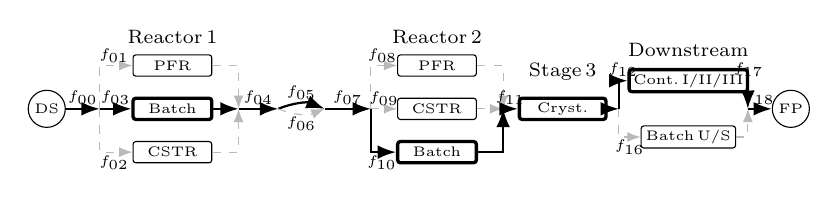
\begin{tikzpicture}[
    x=0.84cm, y=0.55cm,
    opt/.style={-Latex, thick},
    alt/.style={-Latex, thin, dashed, draw=gray!55},
    bbk/.style={-Latex, thick},
    unit/.style={draw, rounded corners=1pt, align=center, inner sep=1.5pt,
        minimum width=1.0cm, minimum height=0.27cm, font=\tiny},
    optunit/.style={draw, very thick, rounded corners=1pt, align=center, inner sep=1.5pt,
        minimum width=1.0cm, minimum height=0.27cm, font=\tiny},
    lbl/.style={font=\tiny, inner sep=1pt}
]
% Source
\node[circle, draw, inner sep=1.5pt, font=\tiny] (DS) at (-0.4, 0) {DS};
% f00 (backbone)
\coordinate (sp1) at (0.4, 0);
\draw[bbk] (DS) -- node[above, lbl] {$f_{00}$} (sp1);
% Reactor 1
\node[unit]    (pfr1)  at (1.5,  1.0) {PFR};
\node[optunit] (bat1)  at (1.5,  0.0) {Batch};
\node[unit]    (cstr1) at (1.5, -1.0) {CSTR};
\node[lbl, font=\scriptsize, above=2pt] at (1.5, 1.3) {Reactor\,1};
\draw[alt] (sp1) |- node[above, lbl, pos=0.72] {$f_{01}$} (pfr1);
\draw[opt] (sp1) -- node[above, lbl]           {$f_{03}$} (bat1);
\draw[alt] (sp1) |- node[below, lbl, pos=0.72] {$f_{02}$} (cstr1);
\coordinate (mg1) at (2.5, 0);
\draw[alt] (pfr1)  -| (mg1);
\draw[opt] (bat1)  -- (mg1);
\draw[alt] (cstr1) -| (mg1);
% f04 (backbone)
\coordinate (sp2) at (3.1, 0);
\draw[bbk] (mg1) -- node[above, lbl] {$f_{04}$} (sp2);
% Routing f05 / f06
\coordinate (mg2) at (3.8, 0);
\draw[opt] (sp2) to[bend left=22]  node[above, lbl] {$f_{05}$} (mg2);
\draw[alt] (sp2) to[bend right=22] node[below, lbl] {$f_{06}$} (mg2);
% f07 (backbone)
\coordinate (sp3) at (4.5, 0);
\draw[bbk] (mg2) -- node[above, lbl] {$f_{07}$} (sp3);
% Reactor 2
\node[unit]    (pfr2)  at (5.5,  1.0) {PFR};
\node[unit]    (cstr2) at (5.5,  0.0) {CSTR};
\node[optunit] (bat2)  at (5.5, -1.0) {Batch};
\node[lbl, font=\scriptsize, above=2pt] at (5.5, 1.3) {Reactor\,2};
\draw[alt] (sp3) |- node[above, lbl, pos=0.72] {$f_{08}$} (pfr2);
\draw[alt] (sp3) -- node[above, lbl]           {$f_{09}$} (cstr2);
\draw[opt] (sp3) |- node[below, lbl, pos=0.72] {$f_{10}$} (bat2);
\coordinate (mg3) at (6.5, 0);
\draw[alt] (pfr2)  -| (mg3);
\draw[alt] (cstr2) -- (mg3);
\draw[opt] (bat2)  -| (mg3);
% Crystallisation (always active)
\node[optunit, minimum width=1.1cm] (cryst) at (7.4, 0) {Cryst.};
\node[lbl, font=\scriptsize, above=2pt] at (7.4, 0.45) {Stage\,3};
\draw[bbk] (mg3) -- node[above, lbl] {$f_{11}$} (cryst);
% Downstream split
\coordinate (sp4) at (8.25, 0);
\draw[opt] (cryst) -- (sp4);
% Continuous downstream (optimal via Cont. I = f13)
\node[optunit, minimum width=1.2cm] (cont) at (9.3,  0.65) {Cont.\,I/II/III};
\node[unit,    minimum width=1.2cm] (bus)  at (9.3, -0.65) {Batch\,U/S};
\node[lbl, font=\scriptsize, above=2pt] at (9.3, 1.0) {Downstream};
\draw[opt] (sp4) |- node[above, lbl, pos=0.75] {$f_{12}$} (cont);
\draw[alt] (sp4) |- node[below, lbl, pos=0.75] {$f_{16}$} (bus);
\coordinate (mg4) at (10.2, 0);
\draw[opt] (cont) -| node[above, lbl, pos=0.25] {$f_{17}$} (mg4);
\draw[alt] (bus)  -| (mg4);
% f18 (backbone) → FP
\node[circle, draw, inner sep=1.5pt, font=\tiny] (FP) at (10.85, 0) {FP};
\draw[bbk] (mg4) -- node[above, lbl] {$f_{18}$} (FP);
\end{tikzpicture}

\smallskip
\textbf{(a)} DS-MFG manufacturing superstructure (19 binary arcs)
\end{minipage}%
\hfill
\begin{minipage}[t]{0.37\linewidth}
\centering
\scriptsize
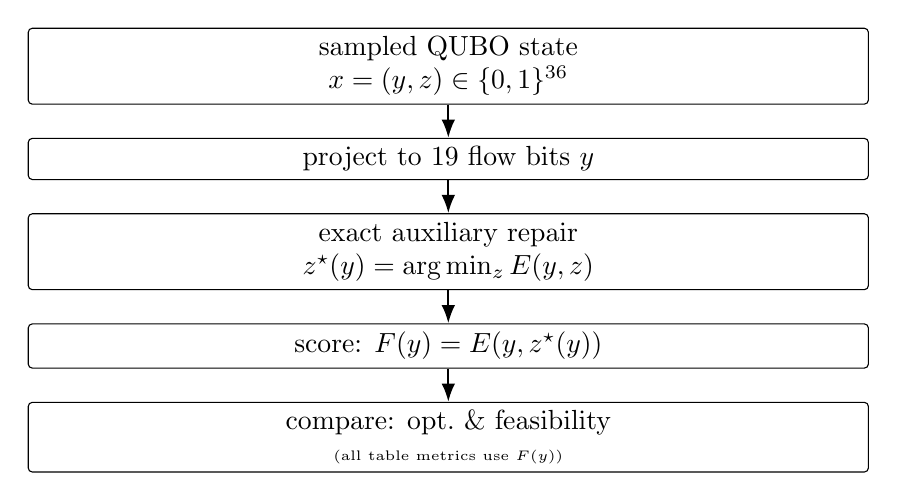
\begin{tikzpicture}[
    node distance=0.42cm,
    box/.style={draw, rounded corners=1.5pt, align=center, inner sep=3pt,
        minimum width=0.88\linewidth},
    arr/.style={-Latex, thick}
]
\node[box] (sample)  {sampled QUBO state\\$x=(y,z)\in\{0,1\}^{36}$};
\node[box, below=of sample]  (project) {project to 19 flow bits $y$};
\node[box, below=of project] (repair)  {exact auxiliary repair\\$z^\star(y)=\arg\min_z E(y,z)$};
\node[box, below=of repair]  (score)   {score: $F(y)=E(y,z^\star(y))$};
\node[box, below=of score]   (compare) {compare: opt.\ \& feasibility\\[-1pt]{\tiny (all table metrics use $F(y)$)}};
\draw[arr] (sample)  -- (project);
\draw[arr] (project) -- (repair);
\draw[arr] (repair)  -- (score);
\draw[arr] (score)   -- (compare);
\end{tikzpicture}

\smallskip
\textbf{(b)} Repair-aware scoring pipeline
\end{minipage}
\caption{Overview of the DS-MFG case study. \textbf{(a)} Manufacturing superstructure: thick arrows trace the optimal flowsheet (Batch\,Rxn\,1\,$\to$\,Route\,A\,($f_{05}$)\,$\to$\,Batch\,Rxn\,2\,$\to$\,Cryst.\,$\to$\,Cont.\,I\,($f_{13}$)); dashed arrows mark the non-optimal alternatives; the backbone arcs $f_{00},f_{04},f_{07},f_{11},f_{18}$ carry every feasible flow. Route~B ($f_{06}$) is activated only when a continuous Reactor~1 feeds a batch Reactor~2; Cont.\,I/II/III share entry arc $f_{12}$ and exit arc $f_{17}$ (optimal uses $f_{13}$). \textbf{(b)} Every sampled 36-bit QUBO string is projected to the 19 flow variables, repaired exactly via the 13-component auxiliary decomposition (GitHub repository), and scored against the certified optimum and the 36-member feasible-design pool; hit rates appear in Table~\ref{tab:ds-mfg-primary-outcomes}.}
\label{fig:ds-mfg-overview}
\end{figure*}

% \begin{figure*}[t]
% \centering
% 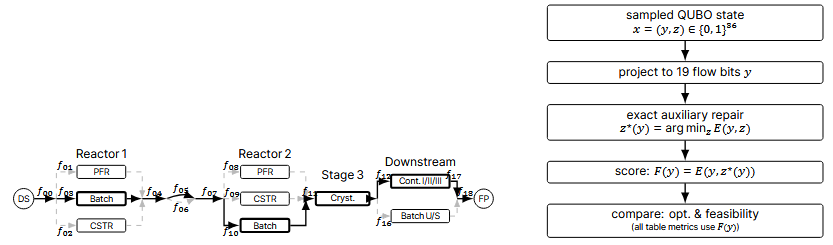
\includegraphics[width=\textwidth]{figure1.png}
% \caption{Overview of the DS-MFG case study. \textbf{(a)} Manufacturing superstructure: thick arrows trace the optimal flowsheet (Batch\,Rxn\,1\,$\to$\,Route\,A\,($f_{05}$)\,$\to$\,Batch\,Rxn\,2\,$\to$\,Cryst.\,$\to$\,Cont.\,I\,($f_{13}$)); dashed arrows mark the non-optimal alternatives; the backbone arcs $f_{00},f_{04},f_{07},f_{11},f_{18}$ carry every feasible flow. Route~B ($f_{06}$) is activated only when a continuous Reactor~1 feeds a batch Reactor~2; Cont.\,I/II/III share entry arc $f_{12}$ and exit arc $f_{17}$ (optimal uses $f_{13}$). \textbf{(b)} Every sampled 36-bit QUBO string is projected to the 19 flow variables, repaired exactly via the 13-component auxiliary decomposition (GitHub repository), and scored against the certified optimum and the 36-member feasible-design pool; hit rates appear in Table~\ref{tab:ds-mfg-primary-outcomes}.}
% \label{fig:ds-mfg-overview}
% \end{figure*}

\section{Introduction}
\label{sec:ds-mfg-introduction}

Discrete choices are often the first barrier in process design.
Before a flowsheet can be simulated or optimized over continuous variables, the designer must commit to a set of mutually exclusive options: which synthesis route to use, which unit operations to include, and which operating modes to run \cite{Mencarelli_2020}.
In pharmaceutical manufacturing, these choices are particularly consequential because route and equipment selection shape cost, yield, and regulatory burden, and because digital design and optimization tools for this sector are comparatively recent \cite{CasasOrozco2021, Laky2022}.
The resulting models are combinatorial, and even modestly sized superstructures generate large discrete search spaces.

Gate-based quantum optimization is one of the emerging tools proposed for this setting.
A gate-based quantum computer operates on quantum bits (qubits) by applying sequences of parameterized gate operations that form a quantum circuit; measuring the circuit returns a binary string, and the circuit parameters, called angles, are tuned so that low-energy strings appear with high probability.
The quantum approximate optimization algorithm (QAOA) \cite{Farhi2014} and the variational quantum eigensolver (VQE) \cite{Peruzzo2014, Cerezo2021} follow this variational paradigm: QAOA uses $p$ alternating cost and mixer layers, and VQE uses a parameterized ansatz circuit (here, a hardware-efficient ansatz); in both cases, a classical optimizer adjusts the angles.
Current hardware is noisy and of intermediate scale \cite{Preskill2018}, and benchmarking surveys stress that a practical quantum advantage for optimization has not yet been established \cite{Abbas2024}; the relevant question is what is required to use these methods today and how their output compares with classical baselines.

Within process systems engineering, quantum computing has been reviewed as an emerging capability \cite{BernalAIChE2022}, and hybrid quantum-classical strategies have been proposed for discrete optimization in process and energy systems \cite{AjagekarYou2019}.
Discrete-design instances have been mapped to the quadratic unconstrained binary optimization (QUBO) form \cite{glover2019} and solved with Ising-based annealing hardware \cite{AjagekarYou2019,park2026arxiv}.
These works establish that the mapping is possible; few examine what happens to the samples after the reformulation, and the gate-based path is less explored than annealing.
Casting a constrained problem as a QUBO introduces auxiliary variables \cite{toqubo:2023} that are bookkeeping rather than design decisions, so a raw quantum sample is not directly interpretable as a flowsheet.
The question is: what does it take to turn gate-based quantum samples into process-design decisions, and how does this compare with classical methods?

We answer this through an end-to-end audit on a single drug-substance manufacturing (DS-MFG) instance, chosen to be small enough to enumerate exactly yet large enough to expose the reformulation and interpretation issues that arise at scale.
Our contribution is a repair-aware audit of the full path from a constrained process-design model to usable gate-based quantum samples.
We find:
(i) raw QUBO samples require projection and exact auxiliary repair before they are interpretable as design candidates;
(ii) a quadratic surrogate over the design variables fits the repaired landscape globally but fails as an optimizer;
(iii) QAOA with angles optimized offline on that surrogate concentrates probability on good flowsheets but does not beat classical baselines;
(iv) these findings hold across the tested penalty weights, surrogate training sets, circuit depths, optimizer budgets, and seeds; and
(v) a hardware run confirms pipeline feasibility without adding advantage.
Because the surrogate and the offline angles are built from exhaustive repair enumeration, feasible only for this small instance, the workflow is a diagnostic benchmark for sample interpretation, not a scalable optimization shortcut.

\section{Methods}
\label{sec:ds-mfg-methods}

\subsection{The Discrete Design Instance}
\label{subsec:ds-mfg-instance}

The DS-MFG instance is the discrete subproblem of a drug-substance manufacturing case study introduced by Park and Bernal Neira~\cite{park2026arxiv}, where a mixed-integer nonlinear design problem is decomposed so that the discrete part is handled by combinatorial solvers and the nonlinear part by simulators.
We keep the same discrete instance but ask what is required to run gate-based optimizers.
The instance is a binary integer program for capital-expenditure selection in the manufacturing superstructure of Figure~\ref{fig:ds-mfg-overview}(a): the 19 binary variables $f_i$, $i \in F$, encode candidate material-flow arcs and unit-operation selections, and the objective is a normalized capital-cost score with arc costs $c_i$ (lower values indicate lower capital expenditure; scaled as in \cite{park2026arxiv}).
The discrete problem has the form
\begin{equation}
\begin{aligned}
\min_{f} \quad & \sum_{i \in F} c_i f_i \\
\text{s.t.}\quad
& \sum_{i \in \mathrm{In}(n)} f_i
  = \sum_{j \in \mathrm{Out}(n)} f_j
    && \forall n \in N, \\
& f_{00} = 1,\quad f_{18} = 1,\\
& (1-f_{01}) + (1-f_{10}) + f_{06} \geq 1,\\
& (1-f_{02}) + (1-f_{10}) + f_{06} \geq 1,\\
& (1-f_{03}) + (1-f_{10}) + (1-f_{06}) \geq 1,\\
& f_{01} + f_{02} + f_{05} \geq 1,\quad f_{05} + f_{10} \geq 1,\\
& f_{17} \geq f_{k},\quad k \in \{13,14,15\},\\
& f_i \in \{0,1\}
    && \forall i \in F .
\end{aligned}
\label{eq:ds-mfg-ip-formulation}
\end{equation}
Eq.~\eqref{eq:ds-mfg-ip-formulation} contains three constraint classes: flow balance at each node $n \in N$, a fixed source arc $f_{00}$ and sink arc $f_{18}$, and logic constraints that enforce a valid flowsheet (the Route~B activation rule, the reactor-route compatibility rules, and the shared exit arc of the continuous downstream options).

Solved with Gurobi \cite{gurobi}, the model (19 binary variables, 20 constraints) returns an optimal capital-cost score of 11.7095; with feasible-solution enumeration enabled (\texttt{PoolSearchMode=2}), all 36 feasible flows are retained in a single deterministic solve (0.073 s).
We treat 11.7095 as the certified global optimum and use it as the reference throughout.

\subsection{From Integer Program to QUBO and Back}
\label{subsec:ds-mfg-qubo-repair}

To run QAOA and VQE, the integer program must be expressed as a QUBO, in which all constraints are folded into a single quadratic objective over binary variables \cite{glover2019, toqubo:2023}.
Inequality constraints require auxiliary (slack) variables; the penalty weights and auxiliary count are not unique, and both affect how faithfully the QUBO represents the original problem \cite{toqubo:2023}.
For this instance, the penalty reformulation introduces 17 auxiliary variables, so the QUBO acts on 36 binary variables.
For a bitstring $x \in \{0,1\}^{36}$, the encoded objective is
\begin{equation}
    E_{\mathrm{QUBO}}(x)
    =
    \ell^\top x + x^\top Qx + b,
    \label{eq:ds-mfg-full-qubo}
\end{equation}
with linear coefficients $\ell$, quadratic coefficient matrix $Q$, and constant offset $b$.
The 36 variables separate into the original flow variables and the auxiliaries,
\(
    x = (y,z), \qquad
    y \in \{0,1\}^{19}, \quad z \in \{0,1\}^{17}.
\)
Only $y$ encodes a design decision; $z$ is bookkeeping, so a sampled 36-bit string does not map directly to a flowsheet.
We make it interpretable by projecting onto $y$ and \emph{repairing} the auxiliaries, that is, choosing the assignment that minimizes the QUBO energy for that flow,
\begin{equation}
    F(y)
    =
    \min_{z \in \{0,1\}^{17}} E_{\mathrm{QUBO}}(y,z).
    \label{eq:ds-mfg-repaired-objective}
\end{equation}
The repair is exact and cheap here because, once $y$ is fixed, the auxiliary-auxiliary coupling graph splits into 13 independent connected components: 9 singletons (one auxiliary bit each) and 4 pairs (two auxiliary bits each).
The singletons correspond to the at-most-one inequality constraints for each decision group and to the downstream flow-balance conditions; the pairs arise from product-linearization inequalities for the Route~B activation rule ($f_{06}=1$ iff Reactor~1 is continuous and Reactor~2 is batch).
Each component is solved by enumeration over its 2 or 4 assignments, so $9\!\times\!2+4\!\times\!4=34$ local evaluations replace enumeration of $2^{17}=131{,}072$ auxiliary states.
The full component table, with auxiliary indices, flow neighbors, and constraint roles, is recorded in the shared code repository (link in Acknowledgments).
The decomposition is specific to this instance (see Discussion).

The repaired minimizer over all $2^{19}$ flows recovers the optimum, and the repaired QUBO scores match the integer-program objective to within $3.1\times 10^{-13}$, confirming that they encode the same objective.
Exact enumeration finds exactly 36 feasible flows, as does the solution pool of Gurobi, and they occupy repaired ranks 1--36.

The repaired objective $F(y)$ is not a quadratic function of $y$, but QAOA and VQE require a QUBO input.
Rather than using the full 36-variable QUBO, which mixes design variables with auxiliaries and requires 36-qubit circuits, we construct a reduced 19-variable QUBO over the design space $y$ by fitting a quadratic surrogate to the repaired landscape,
\begin{equation}
    \widehat{F}(y)
    =
    \widehat{b}
    + \widehat{\ell}^{\top} y
    + y^{\top} \widehat{Q} y ,
    \label{eq:ds-mfg-quadratic-surrogate}
\end{equation}
by unweighted least squares over all $2^{19}$ repaired flows ($R^2 \approx 0.999$).
The surrogate serves only as a compact 19-qubit sampling Hamiltonian; it is never used to certify solution quality, and every reported metric is evaluated after exact repair under $F$.

\subsection{Quantum, Classical, and Hardware Workflows}
\label{subsec:ds-mfg-workflows}

The local QAOA and VQE workflows run through \texttt{QiskitOpt.jl}, a Julia wrapper for Qiskit \cite{JavadiAbhari2024}, with QUBO models constructed via the \texttt{QUBO.jl} ecosystem \cite{toqubo:2023}.
Increasing $p$ makes QAOA more expressive and can be viewed as a finer discretization of an adiabatic path \cite{Farhi2000}, but deeper circuits are more sensitive to noise on current NISQ devices \cite{Preskill2018}.
Direct full-QUBO QAOA and VQE operate on the 36-variable formulation, and reduced-surrogate QAOA and VQE on the 19-variable surrogate; both tune their angles with the native COBYLA optimizer of Qiskit and are scored by exact repair.
Surrogate VQE uses an \texttt{EfficientSU2} ansatz.
The best-performing workflow, which we call \emph{energy-targeted QAOA}, replaces the native angle search by an offline step: the angles are optimized on the surrogate with JuliQAOA \cite{Golden2023JuliQAOA}, which minimizes the expected surrogate energy $\mathbb{E}_{y \sim p_\theta}[\widehat{F}(y)]$ by basin hopping with BFGS local optimization \cite{Cerezo2021}, and are then transferred to a Qiskit circuit for sampling.
The offline search cost is excluded from the call times in Table~\ref{tab:ds-mfg-primary-outcomes}.
As classical baselines, we sample the repaired 19-flow objective by uniform random sampling and by single-bit-flip hill climbing with random restarts.
As a hardware feasibility test, we run a fixed-angle QAOA circuit on the IBM \texttt{ibm\_fez} quantum computer; its angles were optimized offline to concentrate probability on the ten lowest-cost flows rather than on the expected energy.

For each sampled state $x=(y,z)$ we record the raw QUBO energy $E_{\mathrm{QUBO}}(y,z)$, the repaired objective $F(y)$, and the auxiliary gap.
An \emph{optimum hit} means that the repaired flow equals the certified optimal flowsheet, the unique minimum-cost feasible design; a \emph{feasible-design hit} means that it matches any of the 36 feasible flows.
We report both hit rates with two-sided Wilson 95\% intervals; zero-hit rows show the upper endpoint.
The empirical $\mathrm{TTS}_{99}=\tau\lceil\log(0.01)/\log(1-\hat{p})\rceil$ uses the recorded call time per sample $\tau$; zero-hit rows report $\infty$.
These values compare sampling costs and exclude preprocessing.
Evaluations within a search run are not independent trials, and VQE performance varies with the seed, so the intervals and TTS values are descriptive and do not guarantee success across repeated runs.

\section{Results}
\label{sec:ds-mfg-results}

Table~\ref{tab:ds-mfg-primary-outcomes} summarizes the primary outcomes: energy-targeted QAOA gives the highest stochastic feasible-design rate, but hill climbing and Gurobi remain faster on the recorded cost metrics.

\subsection{Repair Changes the Meaning of a Sample}
\label{subsec:ds-mfg-repair-meaning}

Sampling the 36-variable QUBO directly does not yield an interpretable design result.
A $p=2$ full-QUBO QAOA found no optimum in 512 samples; a 32768-read run returned it only 4 times after repair, and never as a fully optimal 36-bit string without projection.
Without projection and exact repair, a raw QUBO sample cannot be read as a flowsheet; Figure~\ref{fig:ds-mfg-overview}(b) summarizes the scoring pipeline.

\subsection{Reduction and Offline Angle Optimization Concentrate QAOA Samples}
\label{subsec:ds-mfg-qaoa-main}

Once the pipeline is in place, reduction to the surrogate and the offline angle search are what make QAOA samples concentrate on feasible, optimal flowsheets.
Energy-targeted QAOA at $p=5$ sampled the certified optimum 664 times in 262144 ideal reads and matched a feasible flowsheet 32502 times (12.4\%, CI [12.3, 12.5]\%), the highest feasible-design rate of any workflow; an independent state-vector calculation puts the optimum probability of this circuit at $2.63\times 10^{-3}$, consistent with the sampled $2.53\times 10^{-3}$.
The near-perfect global $R^2$ of the surrogate did not imply optimization fidelity: its own minimizer repairs to 14.5505 rather than 11.7095, the true optimum ranks only 33rd under the surrogate, and among the 50 lowest-cost repaired flows the absolute surrogate errors reach 29.4.

\subsection{VQE and Classical Baselines Bound the Claim}
\label{subsec:ds-mfg-vqe-classical-main}

VQE benefits from the same reduction but produces a flatter distribution.
Full-QUBO VQE found no optimum in a five-seed sweep.
Table~\ref{tab:ds-mfg-primary-outcomes} reports all 20 initial reduced-surrogate runs, seeds 74001--74020 with 32768 reads each, with 3 optimum and 61 feasible-design hits in 655360 reads; only seeds 74001 and 74007 found the optimum (1 and 2 hits).
Hill climbing found the optimum 19 times in 262144 evaluations; despite a lower hit rate than QAOA, its much smaller per-sample cost gives a better TTS99-opt (0.23 s vs.\ 0.37 s for QAOA).
Random sampling never found the optimum.
Thus, QAOA gives the highest stochastic feasible-design rate but does not beat classical baselines on time-to-solution.

\begin{table*}[t]
\centering
\footnotesize
\caption{Primary outcomes after exact auxiliary repair. Opt rate: certified-optimum hit rate; feas rate: any of the 36 feasible designs. Wilson 95\% intervals [lo,\,hi] use the same units as the rate; zero-hit rows show the upper endpoint. Call time covers the recorded solver call or hardware run. It excludes prior preprocessing and any scoring performed after the call. TTS99 uses these call times and does not measure the full workflow or guarantee success across seeds (Methods). Gurobi reports a deterministic solve time.}
\label{tab:ds-mfg-primary-outcomes}
\setlength{\tabcolsep}{3pt}
\begin{tabular}{L{0.19\linewidth}L{0.07\linewidth}L{0.19\linewidth}L{0.18\linewidth}L{0.09\linewidth}L{0.09\linewidth}}
\hline
Workflow & Call time (s) & Opt rate [95\% CI] & Feas rate [95\% CI] & TTS99-opt (s) & TTS99-feas (s) \\
\hline
Gurobi solution pool & 0.073 & Deterministic optimum & 36/36 (exhaustive) & 0.073 & 0.073 \\
\hline
Uniform random sampling & 2.08 & $<\!1.5{\times}10^{-5}$ & $8.0\,[5.2,\,12.2]{\times}10^{-5}$ & $\infty$ & 0.46 \\
\hline
Hill-climb restarts & 0.93 & $7.2\,[4.6,\,11.3]{\times}10^{-5}$ & $2.75\,[2.56,\,2.96]{\times}10^{-3}$ & 0.23 & 0.006 \\
\hline
Energy-targeted QAOA, $p{=}5$ & 53.9 & $2.53\,[2.35,\,2.73]{\times}10^{-3}$ & $0.124\,[0.123,\,0.125]$ & 0.37 & 0.007 \\
\hline
Reduced-surrogate VQE, all 20 seeds & 45.4 & $4.6\,[1.6,\,13.5]{\times}10^{-6}$ & $9.3\,[7.2,\,12.0]{\times}10^{-5}$ & 69.7 & 3.43 \\
\hline
IBM \texttt{ibm\_fez} pilot & 73.5 & $<\!1.1{\times}10^{-4}$ & $1.1\,[0.42,\,2.8]{\times}10^{-4}$ & $\infty$ & 84.6 \\
\hline
\multicolumn{6}{@{}p{0.99\linewidth}@{}}{\footnotesize\itshape Key counts: QAOA $p{=}5$: 664 opt.\ hits and 32502 feas.\ hits in 262144. IBM \texttt{ibm\_fez}: 0 opt.\ hits and 4 feas.\ hits in 36864.} \\
\end{tabular}
\end{table*}

\subsection{Hardware Execution Is an Implementation Feasibility Check}
\label{subsec:ds-mfg-hardware-main}

To check that the implementation runs on hardware, we submitted the fixed-angle QAOA circuit to the \texttt{ibm\_fez} quantum computer across three repeats and three random transpile seeds (92001--92003), with 4096 measurement shots per repeat, for 36864 total hardware reads (9 jobs, 73.5 s elapsed including cloud queue).
The run produced 4 feasible-design reads and no optimum read; the best hardware sample was the second-cheapest feasible flowsheet (objective 11.8105).
Using this recorded time gives a TTS99-feas of 84.6 s, versus 0.006 s for hill climbing and 0.073 s for the deterministic Gurobi solve.
Queue time was not recorded separately, so we cannot determine how much it contributed.
With zero optimum hits, the Wilson 95\% upper bound on the hardware optimum-hit rate is about $1.04\times 10^{-4}$.

\subsection{Robustness and Additional Classical Baselines}
\label{subsec:ds-mfg-robustness}

We tested how the results change with penalty weights, surrogate training data, QAOA depth, optimizer budget, and random seeds.
The detailed settings, seeds, results, and timings of each run are not included here but are recorded in the shared repository.
For the penalty test, write the QUBO as capital cost $c(y)$ plus penalty $P(y,z)$ and scale only the penalty, $F_\alpha(y)=c(y)+\alpha\min_z P(y,z)$.
Among the tested values, $\alpha = 0.01$, $0.05$, $0.1$, $0.25$, $0.5$, $1$, $2$, and $4$, exact enumeration gives the same certified optimum for $\alpha\geq0.25$; the three smaller weights give infeasible minima.
All feasible designs rank ahead of every infeasible design for tested $\alpha\geq0.5$, and at the submitted weight ($\alpha=1$) the lowest infeasible score exceeds the highest feasible score by 31.3717.
These results apply to this instance with all penalty terms scaled together.

Because exhaustive enumeration is unavailable at larger scale, we also asked whether a surrogate fitted to a sample of flows behaves differently from the full fit.
Surrogates fitted to uniform random subsets of 1024, 8192, and 65536 flows (three seeds per size) reach global $R^2$ values of 0.99884--0.99908, yet their minimizers repair to 14.5505--18.1755 and none identifies the true optimum.
The failure of the surrogate as an optimizer is therefore a property of the quadratic form, not of the training set.

To test the sensitivity of energy-targeted QAOA to circuit depth, initialization, and optimizer budget, we repeated the offline angle search for $p=1$--5 with three random seeds.
The search builds the depth-$(p{+}1)$ starting point from the depth-$p$ solution, so its cost is recorded for the whole $p=1$--5 ladder rather than per depth.
The state-vector optimum probability rises from $1.42\times10^{-4}$ at $p=1$ to $(2.63$--$2.81)\times10^{-3}$ at $p=5$ across seeds.
The optimizer budget is the number of basin-hopping iterations, that is, of random angle perturbations each followed by a BFGS local search; raising it from one to five at one seed leaves the $p=5$ optimum probability at $2.63\times10^{-3}$ while the optimization time for the ladder grows from 103.6 to 300.5~s.
Depth, not optimizer budget, controls the concentration of the samples.

VQE outcomes, in contrast, depend strongly on the seed.
Seed 74018, which had the most top-50 hits in the 20-seed screen (23) but no optimum hit, gave 20 optimum hits when extended to 524288 reads, while seeds 74001 and 74007 gave 5 and 3; reruns of the same three seeds that also retained circuit metadata gave 3, 1, and 0.
A single seed therefore cannot represent VQE performance, and Table~\ref{tab:ds-mfg-primary-outcomes} reports the complete screen.

Finally, we compared simulated annealing~\cite{Kirkpatrick1983}, uniform sampling, and hill climbing using five common seeds and the same 262144-evaluation budget as the QAOA reads in Table~\ref{tab:ds-mfg-primary-outcomes}.
Annealing and hill climbing find the optimum in all five runs (9--25 and 17--27 hits), and uniform sampling in three (at most 1 hit).
Energy-targeted QAOA reaches the optimum more than 20 times as often per read, but each classical run finishes in 0.6--2.3~s, the same order as the hill-climb call time in Table~\ref{tab:ds-mfg-primary-outcomes}, whereas the QAOA sampling call took 53.9~s after 96--105~s of offline angle search.
QAOA therefore yields the most concentrated distribution and the slowest route to the optimum.

\section{Discussion and Limitations}
\label{sec:ds-mfg-discussion}

This study asks what is needed to turn QAOA and VQE samples into meaningful process-design decisions.
The steps are to separate design and auxiliary variables, repair the auxiliaries exactly, fit a quadratic surrogate, optimize the angles offline, and score samples in the original flow space.
Even when the samples concentrate on good flowsheets, classical methods remain faster for this instance.

The call times in Table~\ref{tab:ds-mfg-primary-outcomes} cover only the sampling stage.
A complete quantum workflow also includes reformulation, exhaustive enumeration and repair, surrogate fitting, offline angle optimization, circuit compilation, and, on hardware, queueing and result retrieval.
Timings for these stages were not retained for the original runs, and the 73.5~s hardware record does not separate compilation, queue, and execution, so an end-to-end runtime cannot be reconstructed and the sampling-only TTS values understate the quantum cost.
Reference reruns of the omitted stages are recorded in the repository; the offline angle search alone (96--300~s) exceeds every call time in Table~\ref{tab:ds-mfg-primary-outcomes}, so a full accounting would only widen the classical margin.

Exact enumeration finds the optimum before quantum sampling begins, so these experiments test how to interpret samples after repair.
Repair is cheap here because the auxiliary graph has 13 small components; for a general QUBO, auxiliary repair can itself be NP-hard.
Enumeration and dense state-vector simulation each grow as $2^n$, while repair by component enumeration requires $\sum_c 2^{|c|}$ local assignments.
Larger problems would need approximations whose effects on feasibility and optimality would have to be quantified.
Tests on this one 19-flow instance cannot establish scalability or a total runtime advantage for larger process designs~\cite{Abbas2024}.

\FloatBarrier
\section{Conclusion}
\label{sec:ds-mfg-conclusion}

For this drug-substance manufacturing case study, QAOA and VQE samples become interpretable as process-design decisions only after projection to the flow variables and exact auxiliary repair.
Energy-targeted QAOA concentrates probability on good flowsheets but does not beat classical baselines on any time-to-solution metric (Table~\ref{tab:ds-mfg-primary-outcomes}), and this conclusion is unchanged across the tested penalty weights, surrogate training sets, circuit depths, optimizer budgets, and seeds.
The central lesson is that quantum-sample quality must be evaluated after mapping back to the original process decisions; raw QUBO samples can overstate both feasibility and optimization performance, and honest benchmarks must account for the full preprocessing cost.

\section{ACKNOWLEDGMENTS}
This material is based upon work supported by the Center for Quantum Technologies under the Industry-University Cooperative Research Center Program at the US National Science Foundation under Grant No. 2224960.
Scripts, data files, circuit records, and the component table of the auxiliary repair are archived in the shared repository at \url{https://github.com/SECQUOIA/pse-quantum-discrete-optimization}.

\section{DECLARATION OF USE OF AI}
The authors used generative AI tools to assist with initial code drafting, data-analysis scripting, and draft visualization design. All code, analyses, visualizations, and manuscript text were reviewed, corrected, and revised by the authors, who take full responsibility for the accuracy and integrity of all results.

\section{author identifiers}
Author ORCIDs:

Park: 0009-0008-6629-3308

Bernal Neira: 0000-0002-8308-5016


\pseprintreferences
\pseprintcopyright

\end{document}
